\documentclass[fleqn,10pt]{wlscirep}
\usepackage[utf8]{inputenc}
\usepackage[T1]{fontenc}
\usepackage{listings}
\title{Odysseia: Genetic Regulatory Feature Analysis with Interpretable Classification Machine Learning Models}

\author[1,*1]{Jack Yu}
% \author[1,2,*1]{Jack Yu}
\author[1,]{Jiawang Tao}
% \author[1,*2]{Jie Wang}

% \author[2,+]{Derek Author}
\affil[1]{Affiliation, department, city, postcode, country}
% \affil[2]{Affiliation, department, city, postcode, country}
\affil[*1]{Correspondence: gyu17@alumni.jh.edu}
% \affil[*2]{Correspondence: gyu17@alumni.jh.edu}
% \affil[+]{these authors contributed equally to this work}
\keywords{Cell Reprogramming,Machine Learning,Gene Regulatory Network}

\begin{abstract}
With rapid progress of robust single-cell transcriptome sequnecing since last decade, numerous complicate mechanism underlying cell development has been revealed.
Yet, single-cell RNA sequencing (scRNA-seq) analysis is widely accepted as main approach to define cell stages and phenotypes.
As conversion of somatic cells into induced pluripotency cells already succeeded, identification key genetic factors(GFs) with scRNA-seq for cell reprogramming in biological research and regenerative medicine fields has gained great attention.
Herein, we describe \emph{Odysseia}, an interpretable machine learning classifier based single-cell gene expression profile(scGEP) analysis system, that assesses importances of genetic regulatory features in differentiating cell state(CS).
Furthermore, combined with regulatory network analysis, extracted factors can help to find specific key GFs in implementing CS conversions.
Analyzing 3 published cell reprogramming related reports studying diverge cell types, \emph{Odysseia} correctly extracts genes acclaimed being capable to induce CS conversion.
Overall, \emph{Odysseia} provides an option to obtain guidance information while elucidating mechanism to engineer cellular phenotypes.
\end{abstract}

\begin{document}
\flushbottom
\maketitle
% * <john.hammersley@gmail.com> 2015-02-09T12:07:31.197Z:
%
%  Click the title above to edit the author information and abstract
%
\thispagestyle{empty}
% \noindent Please note: Abbreviations should be introduced at the first mention in the main text – no abbreviations lists. Suggested structure of main text (not enforced) is provided below.
\section*{Introduction}
Since cell reprogramming of mouse embryonic fibroblasts(MEF) to induced pluripotent stem cell(iPSC) succeed in 2006\cite{yamanaka_2006}, several more CS transition methods have been established both in vivo and in vitro\cite{fibroblast_sertoli_2012,fibro_cardio_2012,mef_hept_2011}, spurring prospective development in biomedical area.
However, reprogrammed cells could still fail to flawlessly match in vivo counterparts' identities\cite{ASCL1_dopaminergic_neuron_2021}, and precise reprogramming toward cell subtypes remain impossible\cite{cell_repro_review}.
As gene expression profiles for each individual cell in query population became accessible with scRNA-seq, substantial progress in accurately defining of cell subtypes with marker gene expression has been made\cite{pancreas_subtypes_2016,lung_subtypes_2014}.
Even though multiple computational methods, like \emph{CellNet}\cite{cellnet_2014}, method of \emph{D’Alessio et al}\cite{dalessio_2015}, and \emph{Mogrify}\cite{mogrify_2016}, are already available and proved informativity of determining key transcription factors(TFs) for CS conversion via carrying out novel human cell conversion experiments, limited generalized method could achieve similar goal while utilizing scRNA-seq based expression profiles instead of microarray based or Cap analysis gene expression (CAGE) based databases.
Indeed, constructing scRNA-seq based gene expression database is possible to expand existing methods' applicability in predicting key TFs for cell subtype conversions and elucidating detailed mechanism behind cell reprogramming.
But workload of maintaining complicated database covering majority discovered cell subtypes can be massive; hence, developing generalized scRNA-seq based predictive computational method for determining key GFs in CS conversion with existing methods remain challenging.
In 2019, \emph{SingleCellNet}\cite{scn_2019} is published as successor of \emph{CellNet} in classifying cellular samples with scRNA-seq data but not guiding CS conversion.

Here we present \emph{Odysseia}, a scRNA-seq based expression profile analysis system utilizing interpretablemachine learning classifiers, for not only guiding CS conversion method design but also elucidating mechanisms behind CS conversions.
Unlike previous described methods, \emph{Odysseia} does not require any background expression database but finding potential key GFs in conversing one CS to another with only expression profiles labeled with binary CS categories as input.
Important genetic regulatory pathways(GRPs) being deterministic for classifying CS category will be addressed through assessing and interpreting trained classifiers.
Then, key genes may induce CS conversion will be addressed through analyzing regulons constructed with important GRPs described previously.
The main reason to keep this design is due to consideration on the assumption: The key genes and GRPs may not have converged profiles in either expression or regulatory aspects.
Thus, classification model designed to directly find CS deterministic genes or GRPs can potentially fail to converge on a stable solution.
One of the intuitive approach to solve the non-convergence issue is transforming classification question into higher dimension.
In our case, instead of asking which factors are CS deterministic, we can transform the question into determining CS category, which is supposed to be a converged and labeled profile among input data, with given GEP.
Then, we can analysis the well-performing classifiers and determine which features, equivalent to GRPs, are essential for the classifiers to make correct decisions.

However, in this approach, if a few feature associating with similar functions can be informative enough, CS classifiers could reach remarkably high accuracy with limited features being heavily weighted.
As a result, partial of potential key features will presumably be lost even classifiers being analyzed has demonstrated accuracy over testing data, and informativity of system output will be questionable.
\textbf{
For example, cell growth related genes can also be used as marker genes when separating cells not only in different types but also on distinct cell cycle stages.
But, if only cell growth related genes are found after classifier analysis, system output's capability in guiding CS conversion is unlikely being sufficient.
}
Therefore, a particular classification model designed solving transformed question can still encounter feature lost issue.

In order to overcome feature lost issue as well, \emph{Odysseia} applies multiple classification models with distinct architecture settings in each training iteration then selects well-performing classifiers for further assessment and interpretation.
Through interpreting top-performing classifiers trained with different batches of input data, \emph{Odysseia} enhances the feature extraction capability.

Further details and testing results are discussed in the remainder of this paper which is structured as follow:
\begin{itemize}
\setlength\itemsep{0em}
\item{\hyperref[method]{\textbf{Method:}}}
    firstly, we will summarize the overall system design and describe how it can possibly avoid both non-convergence and feature lost issues.
\item {\hyperref[res]{\textbf{Result:}}}
    secondly, we perform extensive analysis using diverse collection of sequencing data to demonstrate that \emph{Odysseia} can be applied into real world problems, especially in finding potential GFs to perform cell reprogramming.
\item {\hyperref[disc]{\textbf{Discussion:}}}
    third, we discuss about how the outputs of this system can be utilized in further wet lab experiments and what further improvements can be done on this system.
\item {\hyperref[conc]{\textbf{Conclusion:}}}
    finally, we conclude this paper.
\end{itemize}

\section*{Methods}
\label{method}
Briefly, \emph{Odysseia} consists of 4 main steps which can be summarized below and visualized as Figure \ref{odysseia}:
\begin{itemize}
  \item \hyperref[step1]{\textbf{\emph{Step 1}}}: Generate pseudo-celluar gene expression profiles(pseudo-cGEPs) and corresponding pseudo-cellular genetic regulatory network(pseudo-cGRN) with genetic regulatory network(GRN) reconstruction guidance.
  \item \hyperref[step2]{\textbf{\emph{Step 2}}}: Train classification models with GRNs reconstructed with pseudo-cGEPs then select out well-performing models via accuracy evaluation.
  \item \hyperref[step3]{\textbf{\emph{Step 3}}}: Interpret selected classifiers' correct predictions on all generated GRNs.
  \item \hyperref[step4]{\textbf{\emph{Step 4}}}: Perform regulon based analysis on important GRPs found from classifer interpretation in step 3 and extract key genes indicated by the GRPs.
\end{itemize}


\begin{figure}[ht]
\centering
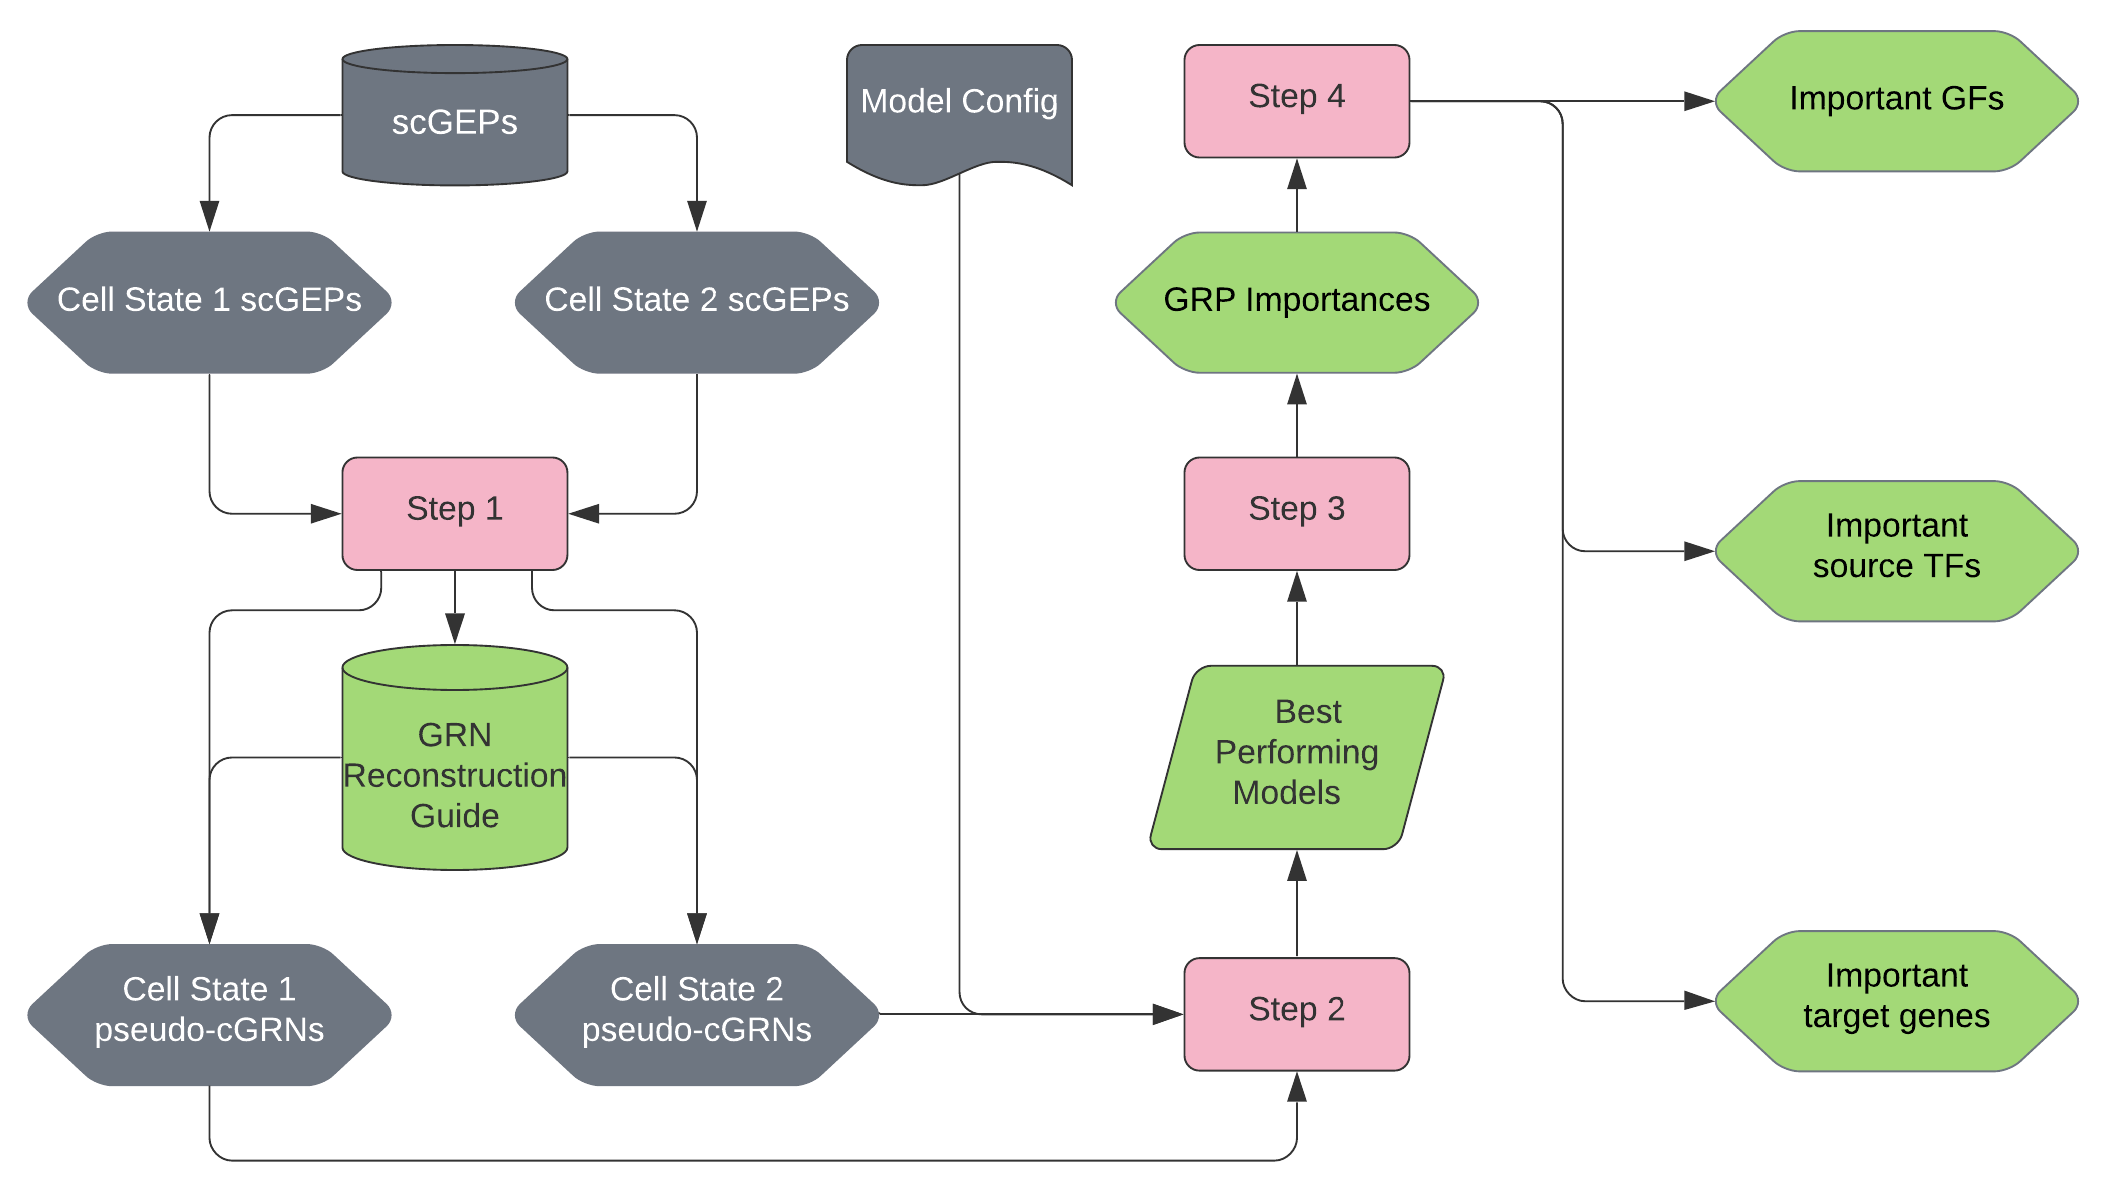
\includegraphics[width=0.8\linewidth]{image/Odysseia.png}
\caption{The overall workflow of \emph{Odysseia}}
\label{odysseia}
\end{figure}


\subsection*{Step 1: Data preprocessing}
\label{step1}
To reconstruct GRNs based on scGEPs, a computational method measurig itenaction strength among gene pairs is mandatory.
One of the widely adopted methods is utilizing pearson correlation coefficient(PCC)\cite{cid_2019, pcc_2012}.
Nevertheless, calculating PCC requires sequence of expression levels(ELs) for each gene amomg interaction rathar than single EL scRNA-seq can provide in one cell.
Hence, in order to reconstruct cell-level GRNs, \emph{Odysseia} segments scGEPs under same CS category into subsets with constant size to form pseudo CEPs, having gene ELs gained from different cells abstracted as sequence of altering ELs among single pseudo cell.

Uncer circumstances scGEPs being scarece, sliding window algorithm(SWA) with customized window size and padding stride can be applied to ensure pseudo-cGEP amount being sufficent for later classifier traning and assessment processes. With SWA, \emph{i-th} pseudo-cGEP can be obtained through:

\centerline{$SWA(i) = \left\{{x_j}_{j = i * s}^{j + l}\right\}, j + l < N$}
Here $N$ denotes for total length of scGEPs gained from scRNA-seq which can be expressed as $\left\{{x_j}_{j = 0}^{N}\right\}$; $l$ denotes for window size; $s$ denotes for padding stride.

Although pseudo-cGRNs will be reconstructed from pseudo-cGEPs respectively, a meta-level process on determining which gene pairs would form regulatory relationships in each pseudo-cGRN can dramatically reduce computational resouce requirement than repeatedly testifying all possible gene pairs in every pseudo-cGEP.
Assuming pseudo-cGEPs have similar expression pattern with comprehensive GEP containing all scGEPs, the GRN reconstruction guidance can be created through analyzing all gene pairs in comprehensive GEP.
The overall workflow to create GRN reconsturction guidance can be summarized as Figure \ref{kirke}.
In total, two sets of filters must be passed for validating a GRP:
\begin{enumerate}
\setlength\itemsep{0em}
\item {\textbf{Gene level}}:

The main purpose of this filter set is confirming whether a gene's expression pattern is differentiable among binary CS categories or not .
\begin{itemize}
\setlength\itemsep{0em}
\item \textbf{Stdev Filter}: The standard deviation(stdev) of gene's EL must be significant.
This filter is to confirm query gene not only can reach relatively high EL but also has expression pattern possibly interacting with other GFs.
By default, the threshold is set to 1 implying that one gene's expression status must be changing in different circumstances to be consudered.

However, stdev threshold would need to be adjusted significantly considering not only significant weight of expression change in studying data but also computational resouce capacity.

\item \textbf{MWU Filter}: The expression distribution of selected gene across samples labeled with different CSs must be dissimilar.
This filter is to confirm query gene's GEP is likely distinguishable across sample sets under binary CS categories.
The Mann-Whitney U rank test(MWU) implemented by \emph{SciPy}\cite{2020SciPy-NMeth} will be performed on GEPs of selected gene in binary CS categories.
By default, the p-value to reject null hypothesis, expression pattern underlying CS1 is the same as the expression pattern underlying CS2, is set to 0.05.
\end{itemize}

\item {\textbf{Pathway level}}:

The main purpose of this filter set is confirming whether a GRP is both biologically interpretable and significant or not.
\begin{itemize}
\setlength\itemsep{0em}
\item \textbf{TF Filter}: The source input of a GRP must be a recorded TF.
If not further specified, TF list will be retrieved from integrated \emph{TRANSFAC}\cite{transfac} datasets according to the specie information in query.
\item \textbf{GRP Filter}: Regulatory target must have binding ability with source TF. If not further specified, regulatory gene list of given TF will be retrieved from integrated \emph{GTRD}\cite{gkaa1057} datasets according to the specie information in query.
\item \textbf{PCC Filter}: Expression correlation between source TF and target gene must be significant. The default setting of threshold is 0.2 for absolute value of Pearson correlation coefficient calculated with \emph{SciPy}\cite{2020SciPy-NMeth}.
\end{itemize}
\end{enumerate}
% In the case of not knowing source $TF's$ correlated binding site information, $GRNBoost2$\cite{grnboost2}-like algorithm will be initiated to predict potential regulatory target.
% The prediction process can either take manually set significant threshold or automatically set threshold based on validated GRPs.
% The process of automated prediction threshold setting can be expressed as:

% \centerline{$Threshold = min(G(E_1, t)\, \uplus \, G(E_2, t))$}

% \noindent Here $G()$ is GRNBoost2\cite{grnboost2}-like algorithm; $E_1$ is subtracted $CL1\;EM$ for GFs passed Gene level filters; $E_2$ is subtracted $CL2\;EM$ for GFs passed Gene level filters; $t$ is the regulatory source $TF$ in most amount of validated GRPs.
\begin{figure}[ht]
\centering
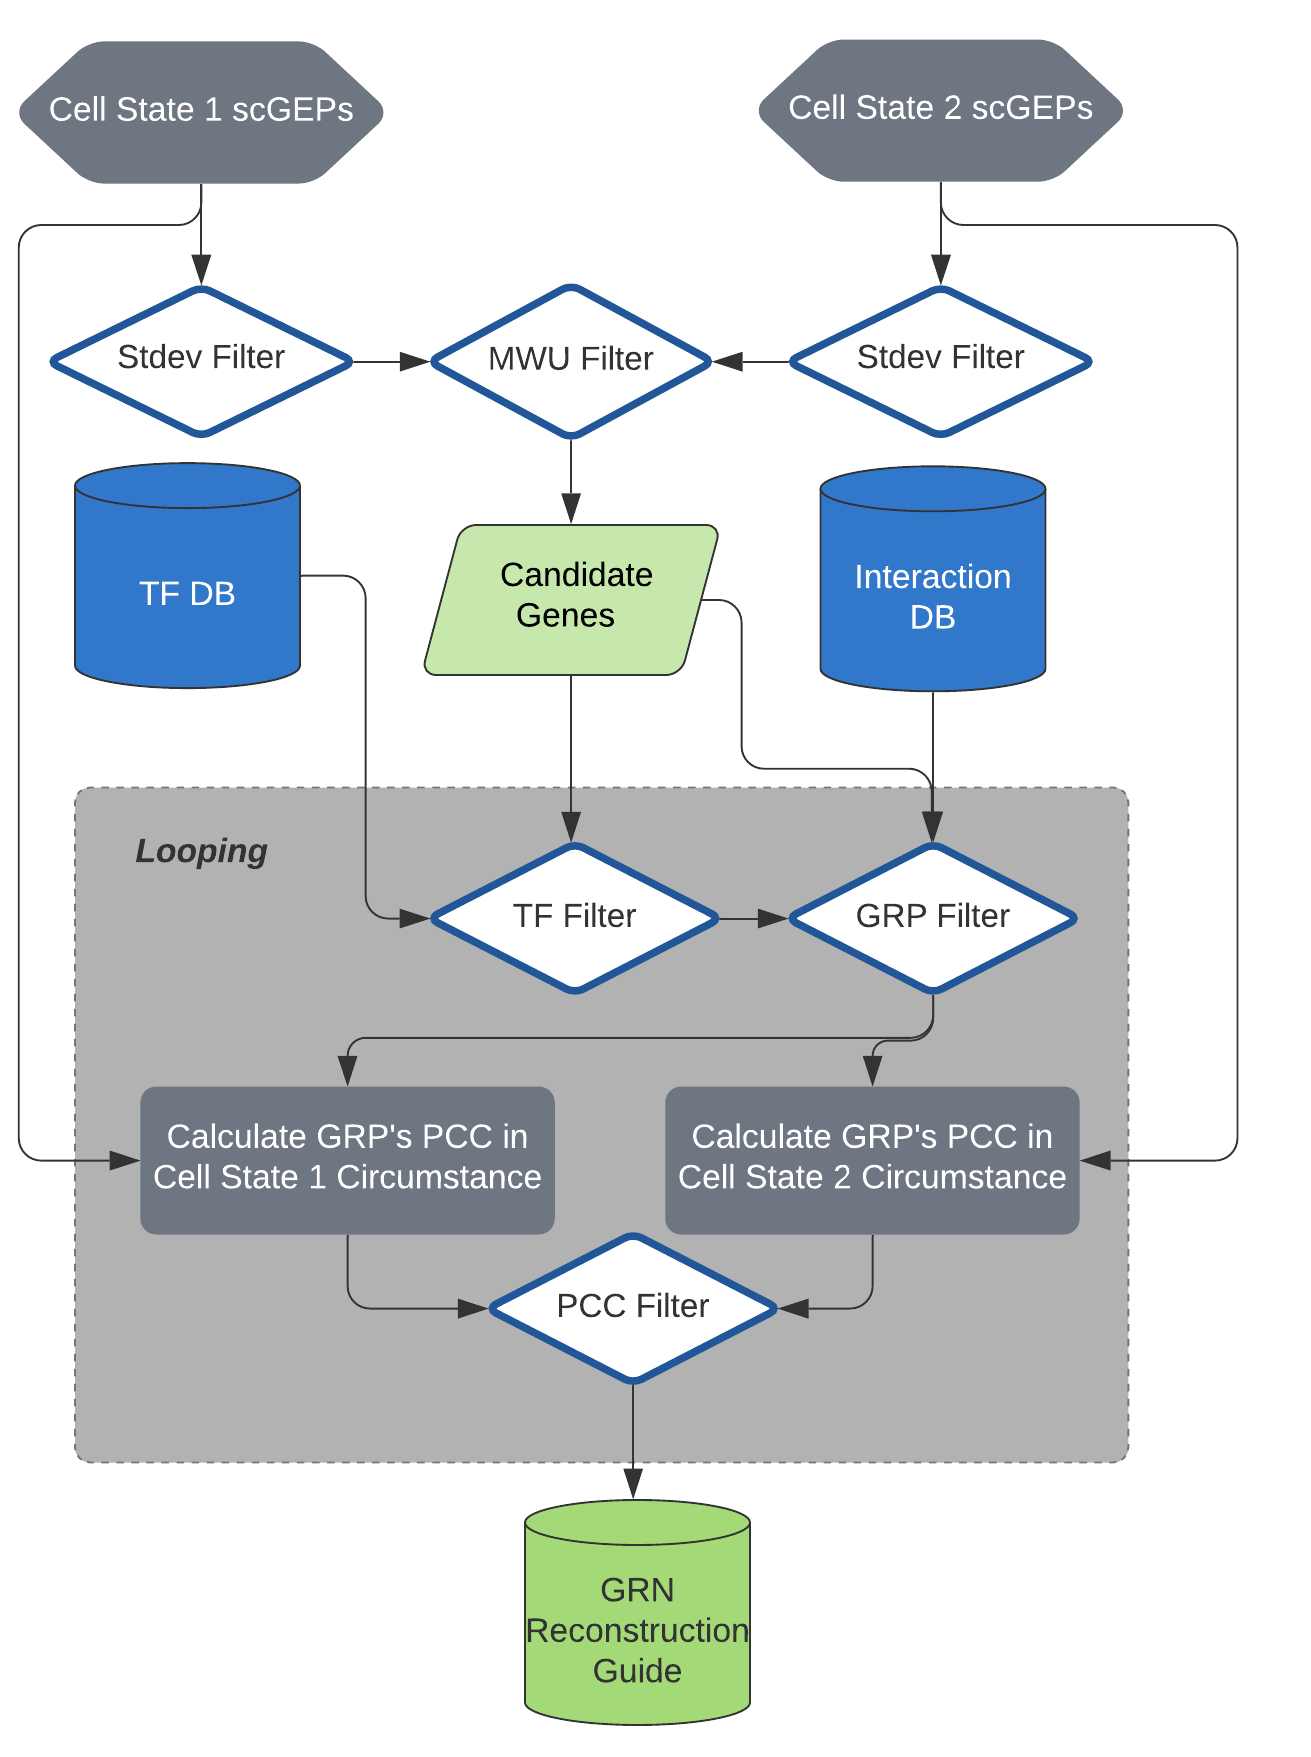
\includegraphics[width=0.8\linewidth, height=12cm, keepaspectratio,]{image/Kirke.png}
\caption{
Workflow to create GRN reconstruction guidance from comprehensive GEPs.
\textbf{\emph{(1)}} Each gene in scGEP set either for CS1 or CS2 need to pass stdev filter confirming its expression pattern is reacting with inconstant gene expression circumstances.
\textbf{\emph{(2)}} GEPs of genes passed stdev filter will be input to MWU filter for confirming gene expression pattern is differentiable among binary CS categories.
\textbf{\emph{(3)}} All TFs in genes passed MWU filter will be selected out as potential regulatory source TF utilizing given TF database.
\textbf{\emph{(4)}} Using GF or protein-protein interaction databae, all genes passed MWU filter will be testified as target genes with potential TF found at previous step to form potential interacting gene pairs.
\textbf{\emph{(5)}}, PCCs of potential interacting gene pairs found previously will be calculated under each CS category. A gene pair must have correspond PCC under at least one CS category greater than threshold to be considered as potential GRP.
}
\label{kirke}
\end{figure}

Utilizing GRN reconstruction guidance, pseudo-cGRN will be reconstructed for each pseudo-cGEP.
Each gene in the guidance, if also presenting in pseudo-cGEP, need to pass the stdev filter in pseudo-cGEP circumstance before validating correspond GRPs in the guidance.
The pre-validated GRPs also passing PCC filter will take part in eventual pseudo-cGRN.

\subsection*{Step 2: Classifier selection}
\label{step2}
According to given model config file, vanilla models will be initialized with specified model type and architecture parameters.
While iterativly training classifiers with split pseudo-cGRN sets, \emph{Odysseia} will also perform accuracy tests systematically aiming to select out potentially well-performing models for further analysis.
The overall workflow can be summarized as Figure \ref{odysseus}.
Currently, \emph{Odysseia} supports three types of classification models:
\begin{itemize}
\setlength\itemsep{0em}
\item \textbf{SVC}: Support Vector Classifer implemented with \emph{scikit-learn}.\cite{scikit-learn}
All parameters adjustable with \emph{scikit-learn}\cite{scikit-learn} are supported.
\item \textbf{GBTree}: Gradient Boosting Trees implemented with \emph{XGBoost}.\cite{chen2016xgboost}
All parameters adjustable with \emph{XGBoost}\cite{chen2016xgboost} are supported.
\item \textbf{CNN}: Convolutional Neural Network implemented with \emph{Pytorch}\cite{NEURIPS2019_9015}.

More specifically, the general architecture designs of \emph{Odysseia}'s integrated CNNs are implemented referring to 1D-CNN and 2D-Hybrid-CNN applied in recent cancer type prediction study\cite{mostavi_chiu_huang_chen_2020}.
Unlike original 1D-CNN and 2D-Hybrid-CNN, we implemented the models with flexibilities not only on kernel related parameters but also on others including amount of convolution layer set which consists a convolution layer and adjacent max-pooling layer.
An example of 1D-CNN with 2 convolution layer sets can be illustrated as Figure \ref{1dCNN}.
\begin{figure}[ht]
\centering
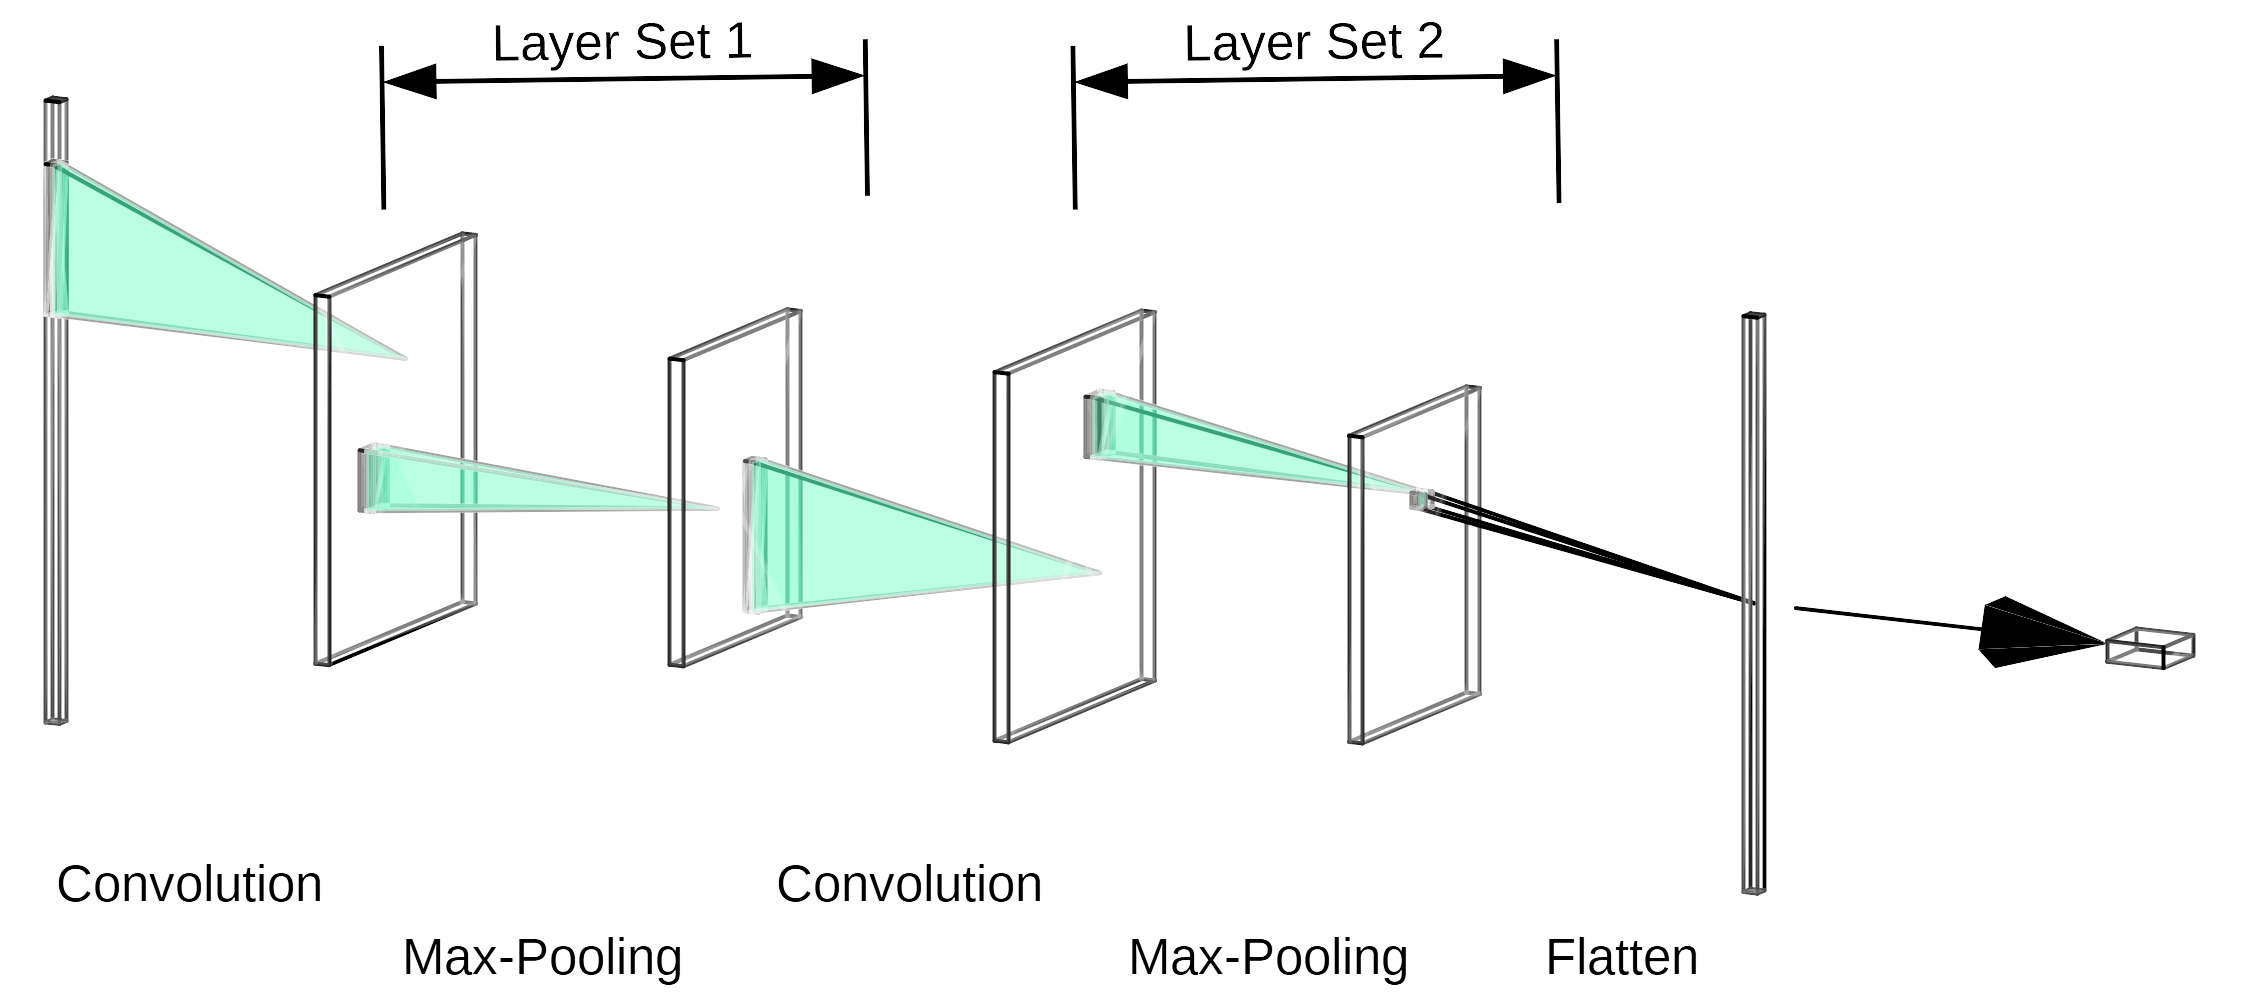
\includegraphics[width=0.8\linewidth]{image/nn.png}
\caption{1D-CNN with 2 convolution layer set.}
\label{1dCNN}
\end{figure}

Other CNNs implemented with \emph{Pytorch}\cite{NEURIPS2019_9015} can also be analyized with \emph{Odysseia} but training protocol need to be clarifed by user in advance.
\end{itemize}

By default model config file, 81 model builds consisting of 1 SVC, 16 GBTrees, and 64 CNNs will be used to initialize vanilla models.
In each training iteration, each vanilla classifier will be fed with same set of pseudo-cGRNs as training samples and primarily assessed according to prediction accuracy on untrained pseudo-cGRNs.
By default setting, at each iteration, 70\% of pseudo-cGRNs will be split into training set while 30\% will be split into testing set.
The classifiers capable of passing accuracy threshold will be kept for further comparisons with other classifers trained with different sample sets in afterward iterations.

At the end of this step, all available pseudo-cGRNs will be joint as testing data, and all candidate classifers will be evaluated on their prediction accuracy of fully joint testing data.
By default, considering the true randomly choosing can reach an accuracy of 50\% in binary classification question, the accuracy threshold for either local accuracy test or fully joint data test is set to 90\%.

\begin{figure}[ht]
\centering
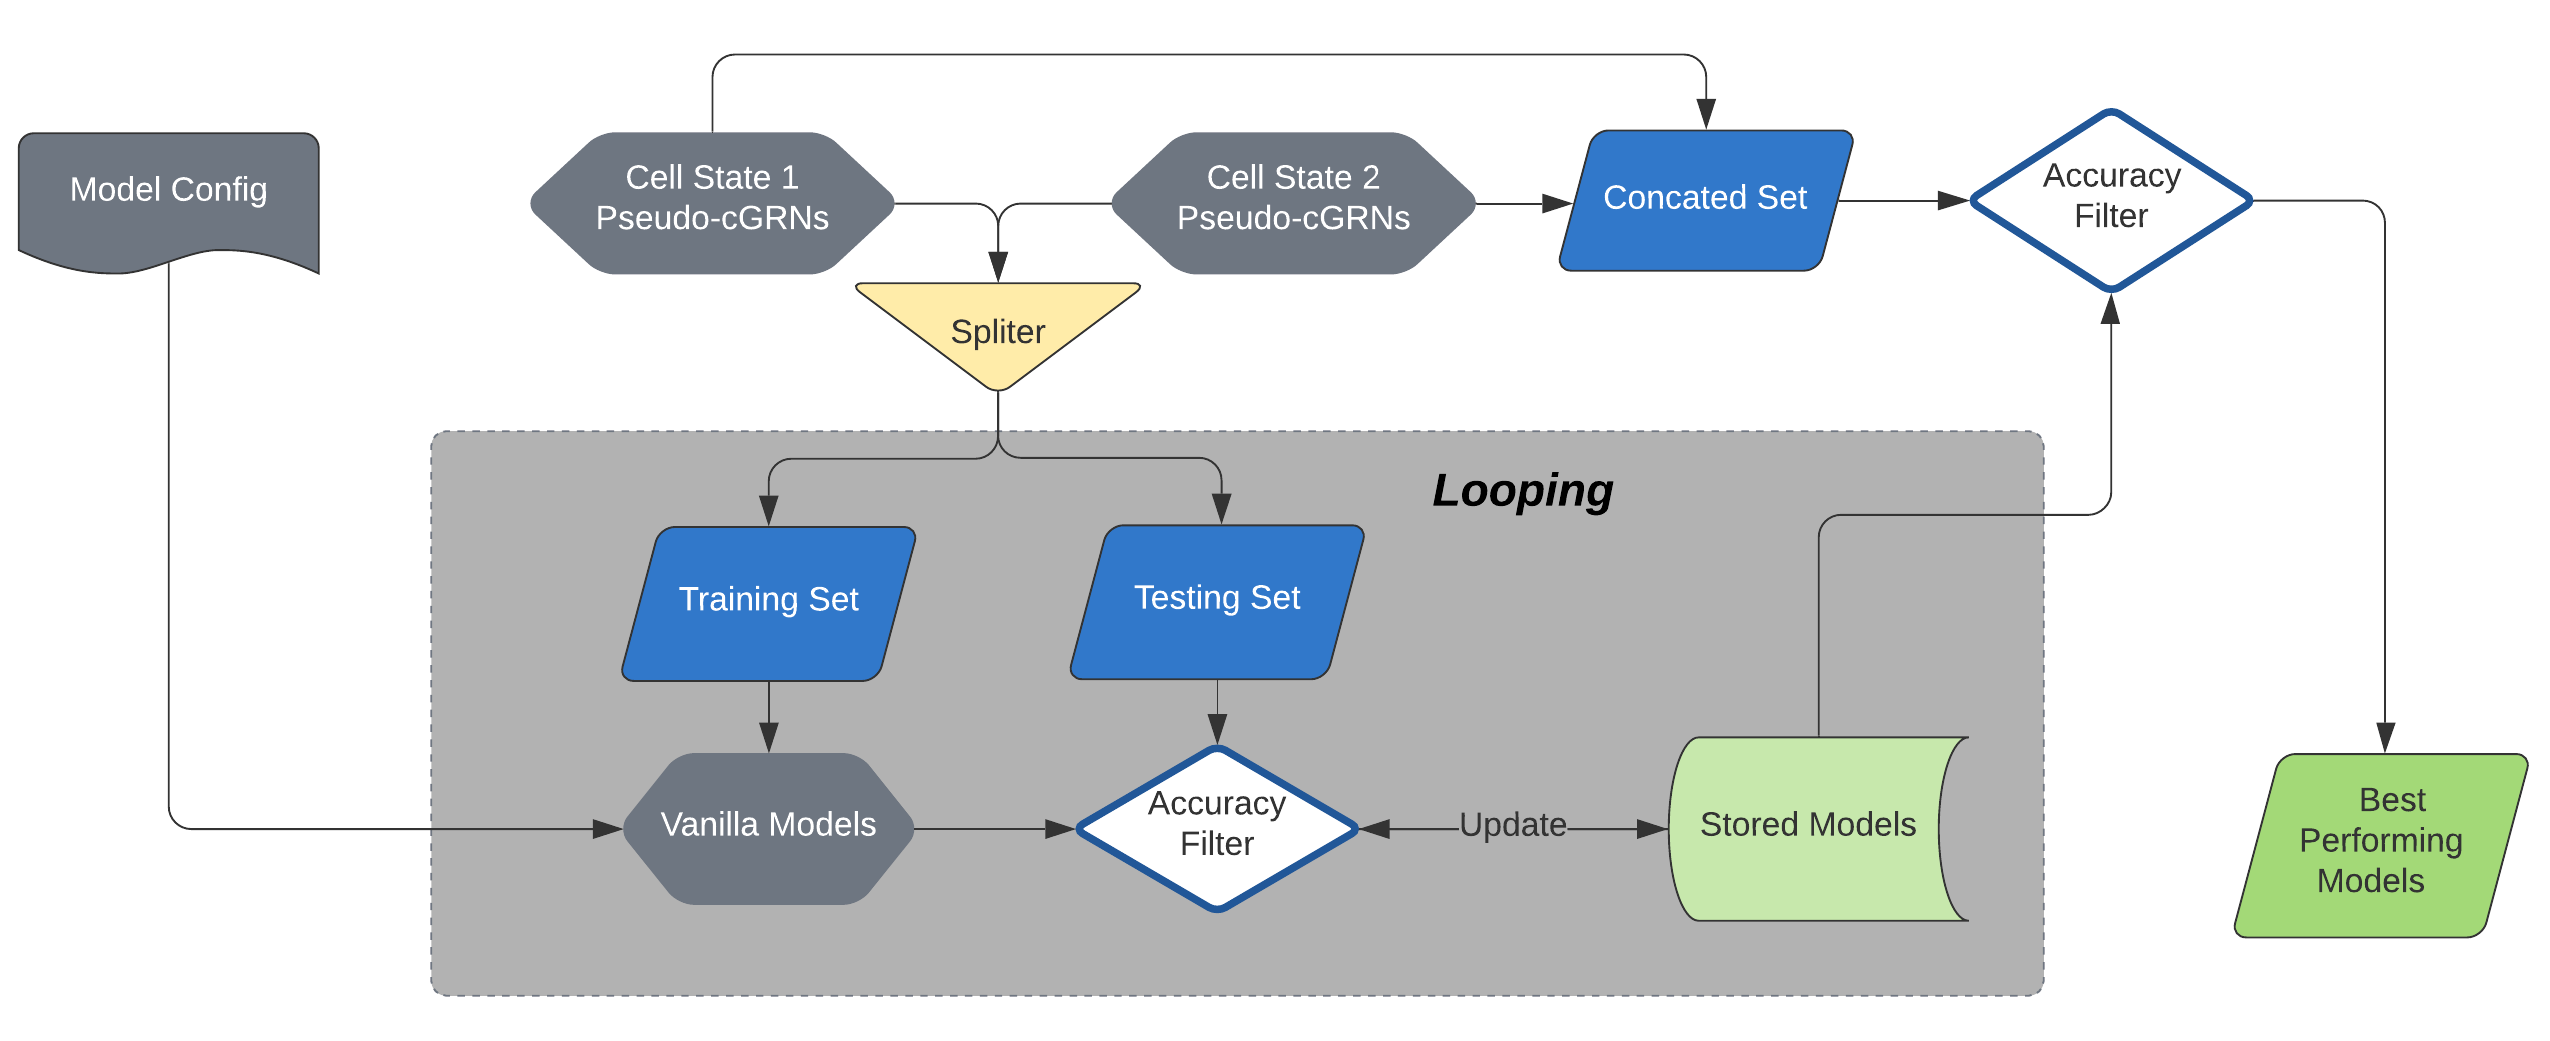
\includegraphics[width=1.0\linewidth]{image/Odysseus.png}
\caption{
Workflow to generate well-performing classifers.
\textbf{\emph{(1)}} In each training iteration, input pseudo-cGRNs will be split into training set and testing set according to given ratio.
By default, the ratio is set to 70\% for training and 30\% for testing.
\textbf{\emph{(2)}} Accoridng to given classification model config file, vanilla classifiers will be initialized and trained with training set.
The predictive accuracy of classifiers will be pre-assessed with testing data.
Classifers reaching accuracy threshold, which is set to 0.9 by default, will be kept for further accuracy assessment in afterward training iterations.
\textbf{\emph{(3)}} After all training iterations, all pseudo-cGRNs will be concated as one testing set to assess accuracies of classifers being kept.
Classifers can still reach accuracy threshold, which is also set to 0.9 by default, will be passed to further analysis.
}
\label{odysseus}
\end{figure}

\subsection*{Step 3: Classifier interpretation}
\label{step3}
During last accuracy assessment in Step 2, all classifer's predictions consisting with ground facts will be marked with corresponding input pseudo-cGRNs.
Briefly, in this step, \emph{Odysseia} interprets how well-performing classifiers make correct predictions on CS categories of given pseudo-cGRNs.
Integrating interpretations of all well-performing classifers, the generalized importance values of features, which are GRPs in \emph{Odysseia}'s scenario, in determining CS can be approached.

To analysis feature importance, several packages already have internalized methods implemented for machine learning models.
For example, GBTree implemented with \emph{XGBoost}\cite{chen2016xgboost} can have feature importance approached through calculating average weight gain at each split involving the feature, and linear SVC implemented with \emph{scikit-learn}\cite{scikit-learn} can have the importance approached with feature coefficient.
Regarding the standard differences between these internalized methods, we utilize \emph{softmax} function to normalize feature importance and define the normalized importance calculation function as:

\centerline{$\textit{T(Z) = }\left\{\frac{f(Z_i)}{\sum_{j = 1}^{L} f(Z_j)}\right\}, i \in Z$}

\noindent Here $Z$ is feature set; $L$ is total number of features; $f(X)$ is internalized  feature importance calculating function of classification model.\

However, for numerous machine learning models, there is no internalized feature importance approaching method, for example NN based models implemented with Pytorch\cite{NEURIPS2019_9015}, or generalized method cannot be appropriately applied with selected models, such as Kernelized SVC implement with \emph{scikit-learn}\cite{scikit-learn}.
Therefore, we apply the concept of The Shapley value\cite{roth_1988} to build an universal approach for determining importance of each feature in any kind of machine learning model.
Specific Shapley value calculation or approaching methods are implemented with \emph{SHAP}\cite{lundberg2017unified} and applied to different types of classifiers as shown in Table\ref{shap}.

\begin{table}[ht]
\centering
\begin{tabular}{|l|l|l|}
\hline
\textbf{Model Genera} & \textbf{Model Example} & \textbf{SHAP\cite{lundberg2017unified} Method}  \\
\hline
Tree-Based & GBTree & Tree Explainer \\
\hline
NN-Based without Repetitive Layer Sets & CNN & Deep Explainer \\
\hline
NN-Based with Repetitive Layer Sets & Recurrent Neural Network & Gradient Explainer \\
\hline
Kernel Machines & SVC & Kernel Explainer \\
\hline
Linear Models & Logistic Regression & Linear Explainer \\
\hline
\end{tabular}
\caption{\label{shap}Machine learning model generas with applicable Shapley value approaching methods}
\end{table}

Let $N$ denoting total number of correct predictions, $\phi_{x,j}^{i}$ and $\phi_{y,j}^{i}$ denoting Shapley value of feature $i$ when predicting sample $j$ as type $x$ or type $y$, the function determining importance values of feature set $z$ can be expressed as:

\centerline{$\textit{T(Z) = softmax}(\left\{\sum_{j = 1}^{N}\frac{\left|\phi_{x,j}^{i}\right| + \left|\phi_{y,j}^{i}\right|}{2}\right\}, i \in Z)$}

Following analysis all classifers, each feature's general importance value can be obtained through:

\centerline{$g(i) = \sum_{j = 1}^{C}T_{j}(Z)[i]$}

Here $i$ denoting \emph{i th} feature or GRP, $C$ denoting total number of classifers being analyzed, $T_{j}(Z)[i]$ denoting \emph{i th} feature's importance value calculated through analyzing \emph{j th} classifier.

\subsection*{Step 4: Key genes extraction}
\label{step4}
With feature list ranked according to importance values, \emph{Odysseia} reconstructs a regulon for top ranked GRPs and extracts influential genes among the regulon.
If analoging regulon or GRN with the graph concept in discrete mathematics, one of the most common methods to analysis influence of a vertex, which is equivalent with a gene, is assessing correspond degree of the vertex.
Although the regulatory source and target within a GRP can be determined if utilizing interaction database, such as \emph{GTRD}\cite{gkaa1057}, showing regulatory relationship of interactors, numerous computational prediction method, \emph{GRNBoost2}\cite{grnboost2} for example, and comprehensive interaction database, \emph{BioGRID}\cite{biogrid} for example, could not provide faithful indication on regulatory directions.
Consequently, based on choice of interaction database for \emph{Odysseia}, the regulon reconstructed cannot be guaranteed to be a directed graph but can surely be analyzed as undirected graph.
Therefore, in this step, \emph{odysseia} primarily extracts genes with high degrees in the regulon regardless in-degree or out-degree.
To limit total amount of output key genes, the default setting of \emph{Odysseia} is reconstructing regulon for top 100 GRPs, and genes with degree higher than 2 in the regulon will be considered as influential.
If regulatory relationships can be clarifed, the regulatory sources being capable to regulate multiple key genes and the regulatory targets being influenced by mulitple key genes can also be extracted according to GRN reconstruction guidance.

In the circumstance of finding genes can potentially induce CS conversion, referring \emph{Mogrify}\cite{mogrify_2016}, genes being either CS deterministic or capable of regulating key genes shall gain attention.
By default setting, if a gene is not marked important, it must be capable to regulate more than 2 listed key genes to be considered as an important regulatory interactor.

% Both non-convergence issue and feature lost issue reflect on one of the key problems for $AutoML$: "No single machine learning method performs best on all datasets".\cite{NIPS2015_11d0e628}
% Even though this problem can be solved while viewing $AutoML$ as a $CASH$ problem \cite{thornton2013auto}, such approach may not be directly deployable in our scenario considering comprehensive CS deterministic GFs or GRPs could be hardly labeled out.
% Hence, in contrast with directly automating key features finding process, we decide to partially automate CS classification process and export candidate components of joint algorithm to feature importance analysis.
% Compared with applying a particular $ML$ model, $CASH$ solving process during automation have higher potential to utilize comprehensive key features instead limited set of them.
% Furthermore, due to the network-based essence of \emph{Odysseia}, some CS deterministic features failed to be detected after classification model analysis, if having close regulatory relationships with multiple confirmed GFs, can still be traced down during regulon-based analysis at post stage analysis.
%
% \subsection*{Construct Pipeline with Odysseia Modules}
% Utilizing modules stated above, a generalized feature extraction pipeline, $Homeros$ which can be summarized as Figure \ref{odysseia}, has been built.
% At first stage of $Homeros$, a $GRN$ reconstruction guidance will be cast with all available data applying $Kirke$ module.
% Next, $Odysseus$ will be initialized with model config file and train out well-performing models for $CL$ classification.
% Models output by $Odysseus$ will then be analyzed with $Penelopeia$ module to propose important GFs and associated GRPs.
% According to changes in abundant GFs among significant GRPs found by $Penelopeia$, program will determine whether another iteration of training or early stopping shall be performed.
% Once looping part either reaches iteration time limit or be early stopped, latest feature importance table will be used to finalize abundant GFs.
% Finally, regulon analysis will find common source regulators and targeting genes of the abundant GFs and generate candidate GF table.

\section*{Results}
\label{res}
In order to evaluate analytics power, we tested \emph{Odysseia} with 3 previously published CS conversion related scRNA-seq datasets.
Considering the differences in information availability and data size among datasets, each dataset was analyzed with adjusted process:
\begin{itemize}
\setlength\itemsep{0em}
\item \textbf{MEF and ESC}:
This dataset has been used to study cell fate continuum when reprogramming MEF into iPSC, one of the most well-studied CS conversions.\cite{mef_ipsc_cas}
To simulate the process of finding gene combination for reprogramming somatic cell into pluripotent stem cell, we used scGEPs labeled MEFs and embryonic stem cells(ESCs) as input of \emph{Odysseia}.
Due to the limited amount of scGEPs, SWA with window size set to 10 and padding stride set to 1 was applied to generate 73 ESC pseudo-cGEPs and 65 MEF pseudo-cGEPs.
Stdev threshold was set to 100, which resulted in GRN reconstruct guidance consisting 72440 GRPs, in concerning computational load our testing device could accept.
While all other parameters remained at default, \emph{Odysseia} extracted 16 key genes and 9 common regulatory sources of key genes.
Partial key genes which have already been reported in other studies are listed in below, and complete output gene list is included as \textbf{Supplementary Table 1}.

\begin{table}[ht]
\centering
\begin{tabular}{|l|l|l|l|}
\hline
\textbf{Gene} & \textbf{Occurrence} & \textbf{Degree} & \textbf{Previous report}  \\
\hline
Nanog & 16 & 0 & Can reprogram MEF into iPSC with other GFs\cite{ips7f, oct4_nanog_sox2_lin28, oct4_nanog_sox2} \\
\hline
Esrrb & 10 & 0 & Can reprogram MEF into iPSC with other GFs\cite{ips7f, LIF_esrrb, gtmEsrrb_iPSC, JARID2_PRDM14_ESRRB_SALL4A} \\
\hline
Sall4 & 10 & 0 & Can reprogram MEF into iPSC with other GFs\cite{ips7f, JARID2_PRDM14_ESRRB_SALL4A} \\
\hline
Tfcp2l1 & 8 & 0 & Key regulatory mediator supporting ESC identity\cite{tfcp2l1_1, tfcp2l1_2} \\
\hline
Pou5f1 (Oct4) & 7 & 0 & Can reprogram MEF into iPSC with other GFs\cite{yamanaka_2006, oct4_nanog_sox2_lin28, oct4_nanog_sox2, ips2f, ipsOK, osk} \\
\hline
Fos & 3 & 2 & Subunit of AP-1 which can prohibit iPSC reprogramming\cite{ips7f, ipsAP1} \\
\hline
Klf4 & 2 & 0 & Can reprogram MEF into iPSC with other GFs\cite{yamanaka_2006, ips2f, ipsOK, osk} \\
\hline
\end{tabular}
\end{table}

Here, \textbf{Occurrence} refers to occurrences in top ranked GRPs; \textbf{Degree} refers to amount of regulating key genes; \textbf{Previous report} summarizes key findings from previous reports.

\item \textbf{MEF and iMPC}:
The main purpose of analyzing this dataset is to assess \emph{Odysseia}'s peformance while stimulating natural cells with artificially induced cells.
This dataset is retrieved from research project studying detailed processes of fibroblast to myocyte and myogenic progenitor cell(MPC) conversion.\cite{mef_iMPC_ETH}
For approaching muscle cell reprogramming, the output goal of this analysis is designed to find key genes for converting MEF into myoblast and further derived myotube both can be stimulated with MyoD+ induced MPCs(iMPCs)\cite{mpc_as_myoblast}.
Practically, only iMPC scGEPs having EL of Myod1 greater than 1, the lowest positive EL in dataset, were extracted as myoblasts and myotubes co-culture and analyzed with MEF scGEPs.
Due to the computational limitation on our device, pseudo-cGEPs were generated with every 100 scGEPs.
As a result, in total of 99 MyoD+ iMPC and 62 MEFs pseudo-cGEPs were generated.
Stdev threshold was also set to 5 to limit the size of GRN reconstruct guidance being 3756 GRPs.
Without any change on other default parameters, \emph{Odysseia} extracted 6 key genes and 3 common regulatory sources of key genes.
Partial analysis result is listed below under same format as mentioned in section above, and complete output gene list is included as \textbf{Supplementary Table 2}.

\begin{table}[ht]
\centering
\begin{tabular}{|l|l|l|l|}
\hline
\textbf{Gene} & \textbf{Occurrence} & \textbf{Degree} & \textbf{Previous report}  \\
\hline
Sox4 & 73 & 2 & Myogenesis mediator\cite{sox4_2013, myogenic_repro_2018} \\
\hline
Mef2c & 23 & 3 & Synergy factor of MyoD in the conversion of MEF into myoblast\cite{mef2_2017, mef2_skeletal}\\
\hline
Myog & 2 & 4 & Marker of differentiating myoblast\cite{myog_1996, myog_2017} \\
\hline
Tcf4 & 2 & 2 & Marker of MEF in muscle connective tissue; Myogenesis mediator\cite{tcf4_2011, tcf4_2016, tcf4_2017}\\
\hline
Mef2a & 0 & 3 & Synergy factor of MyoD in the conversion of MEF into myoblast\cite{mef2_2017, mef2_skeletal}\\
\hline
Myod1 & 0 & 3 & Can reprogram MEF into myoblast and myotube solely\cite{mef_iMPC_ETH, myod_1990} \\
\hline
\end{tabular}
\end{table}

\item \textbf{iPSC and Dopaminergic Neuron}:
The main purpose of analyzing this dataset is to assess \emph{Odysseia}'s peformance while stimulating natural cells with artificially induced cells.
This dataset is retrieved from research project studying detailed processes of fibroblast to myocyte and myogenic progenitor cell(MPC) conversion.\cite{ips_neuron_ascl1}
Since authors did not provide scRNA-seq data for natural MPCs but only induced MPCs(iMPCs) generated with MyoD dependent treatments, we stimulate natrual MPCs with iMPCs expressing Myod1.
Specifically, only iMPC scGEPs having EL of Myod1 greater than 1, the lowest EL in dataset, were analyzed with MEF scGEPs.
Due to the limitation on our device, pseudo-cGEPs were generated with every 100 scGEPs.
As a result, in total of 99 MyoD+ iMPC and 62 MEFs pseudo-cGEPs were generated.
Stdev threshold was also set to 5 to limit the size of GRN reconstruct guidance being 3756 GRPs.
While all other parameters remained at default, \emph{Odysseia} extracted 6 key genes and 3 common regulatory sources of key genes.
Partial analysis result is listed below under same format as mentioned in section above, and complete output gene list is included as \textbf{Supplementary Table 3}.

\begin{table}[ht]
\centering
\begin{tabular}{|l|l|l|l|}
\hline
\textbf{Gene} & \textbf{Occurrence} & \textbf{Degree} & \textbf{Previous report}  \\
\hline
Ets2 & 48 & 12 & ummm\cite{} \\
\hline
Isl1 & 23 & 4 & ummm\cite{}\\
\hline
Ascl1 & 16 & 13 & umm\cite{ips_neuron_ascl1} \\
\hline
Nr3c1 & 0 & 9 & ummm\cite{}\\
\hline
Rbpj & 0 & 8 & ummm\cite{}\\
\hline
Neurod1 & 0 & 7 & ummm\cite{ips_neuron_ascl1} \\
\hline
\end{tabular}
\end{table}

\end{itemize}

Even though \emph{Odysseia} is unable to guarantee a gene combination inducing CS conversion, numerous previously discovered key genes can be successfully extracted and indicate gene combination known capable to convert CSs.
For example, when analyzing MEF with iPSC, the top 3 genes having most occurrences among important GRPs are determined as key factors to reprogram MEF into iPSC with 7F combination\cite{ips7f}.
With Jdp2 which is selected to block AP-1 activity also as Fos indicating, the combination of Jdp2, Nanog, Esrrb, and Sall4 is demonstrated as a minimum 4F functional set to perform cell reprogramming\cite{ips7f}.
While Sall4 indicating interaction between Sox2 and Oct4\cite{sall4_oct4_sox2}, main components among Yamanaka factors\cite{yamanaka_2006, osk} can also be extracted with \emph{Odysseia}'s analysis result.


\section*{Discussion}
\label{disc}
Considering the variability of available types of data in different studies, $Odysseia's$ modules not only can be adjusted upon available resources but also, in order to improve biological interpretability on outputs, provide processed generalized background datasets, such as $GTRD$\cite{gkaa1057} for finding potential target genes of selected transcription factors when building $GRN$ reconstruction guidance. Admittedly, generalized background datasets can still fail to provide substantial support in boundary cases like studying specie is not covered in the dataset. To achieve optimized biological interpretability, substituting generalized dataset with case specific data would be essential.

% Maybe I should also talk about how modifications shall be made as well?

% And how to carry out further analysis with the output stuffs?

\section*{Conclusion}
\label{conc}
Conclusion goes here

\bibliography{reference}

% For data citations of datasets uploaded to e.g. \emph{figshare}, please use the \verb|howpublished| option in the bib entry to specify the platform and the link, as in the \verb|Hao:gidmaps:2014| example in the sample bibliography file.

\section*{Author contributions statement}
\textbf{J.Y.}: Methodology, Software, Writing- Original draft preparation
\textbf{J.T.}: Writing - Review \& Editing
% J.W.: Project administration

\section*{Additional information}
Result, Discussion, Conclusion are not done yet


\subsection*{Key Resource Table}

% \begin{tabular}{|l|l|l|}
%   \hline
%   \textbf{Resource}     & \textbf{Source}     & \textbf{Identifier}\\
%   \hline
%   \textbf{MEF and ESC scRNA-seq data}   & Gene Expression Omnibus Accession: GSE103221 & \url{https://www.ncbi.nlm.nih.gov/geo/download/?acc=GSE103221&format=file&file=GSE103221%5Fnormalized%5Fcounts%2Ecsv%2Egz}\\
%   \hline
%   \textbf{MEF and Myoblast scRNA-seq data}   & Gene Expression Omnibus Accession: GSE169054 & \url{}\\
%   \hline
%   \textbf{iPSC and Neuron scRNA-seq data}   & Gene Expression Omnibus Accession: GSE185275 & \url{}\\
%   \hline
% \end{tabular}



% $CASH$        & Combined Algorithm Selection and Hyperparameter optimization\\
\end{document}
